\chapter{Abgeleitetes Handlungsmodell}\label{ch:handlungsmodell}

Da Methoden zur Sicherung der Vertraulichkeit einen Mehraufwand verursachen und möglicherweise sogar die Qualität von Modellen verschlechtern, sollten diese Methoden nur eingesetzt werden, wenn diese sachgerecht erscheint. 
Abbildung \ref{fig:handlungsmodell} zeigt einen Entscheidungsbaum, welcher bei dieser Fragestellung unterstützt.
Der Entscheidungsbaum wird aus Sicht eines Unternehmens beschrieben, welches Daten sammelt und damit eine Anwendung entwickelt und bereitstellt.
Die einzelnen Kriterien sind dennoch auf Einzelpersonen, öffentliche Open-Source-Projekte oder andere Use Cases anwendbar.
Zudem werden nur die in den vorherigen Kapiteln beschrieben Methoden im Entscheidungsbaum berücksichtigt. 
Grundlegende Sicherheitsmechanismen der Softwareentwicklung, wie \zB Authentifizierung, sollten zusätzlich genutzt werden.

Um den benötigten Schutz von Daten zu ermitteln, sollten Daten in unterschiedliche Vertraulichkeitsstufen klassifiziert werden.
Die Vertraulichkeitsstufen können dabei für jedes Unternehmen individuell sein.
Laut dem Bundesamt für Sicherheit in der Informationstechnik werden Daten häufig wie folgt abgestuft \cite{bsi_200_2}:
\begin{compactitem}
    \item \textbf{Offen}: Diese Daten sind öffentlich bekannt. Diese finden sich beispielsweise auf der öffentlichen Website eines Unternehmens.
    \item \textbf{Intern}: Interne Daten sind Daten, welche unter normalen Mitarbeitern des Unternehmens bekannt und einsehbar sind. Diese könnten beispielsweise in einem Intranet vorhanden sein. Die Daten und Informationen sollten möglichst im Unternehmen bleiben, jedoch würde kein signifikanter Schaden entstehen, wenn diese öffentlich bekannt werden.
    \item \textbf{Vertraulich}: Daten, die vertraulich klassifiziert sind, stehen nur einer definierten Personenmenge zur Verfügung. Eine Veröffentlichung dieser würde dem Unternehmen schaden. Dabei kann der öffentliche Ruf des Unternehmens geschädigt werden, aber auch finanzielle und rechtliche Folgen sind möglich.
    \item \textbf{Streng vertraulich}: Streng vertrauliche Daten stehen ebenfalls nur einer definierten Personenmenge zur Verfügung, wobei die Größe der Personenmenge möglichst gering gehalten wird. Werden diese Daten öffentlich, entsteht ein großer Schaden. Dieser hat in der Regel sowohl rechtliche als auch finanzielle Folgen und schädigt das Unternehmen nachhaltig.
\end{compactitem}

\begin{figure}[!htb]
    \centering
    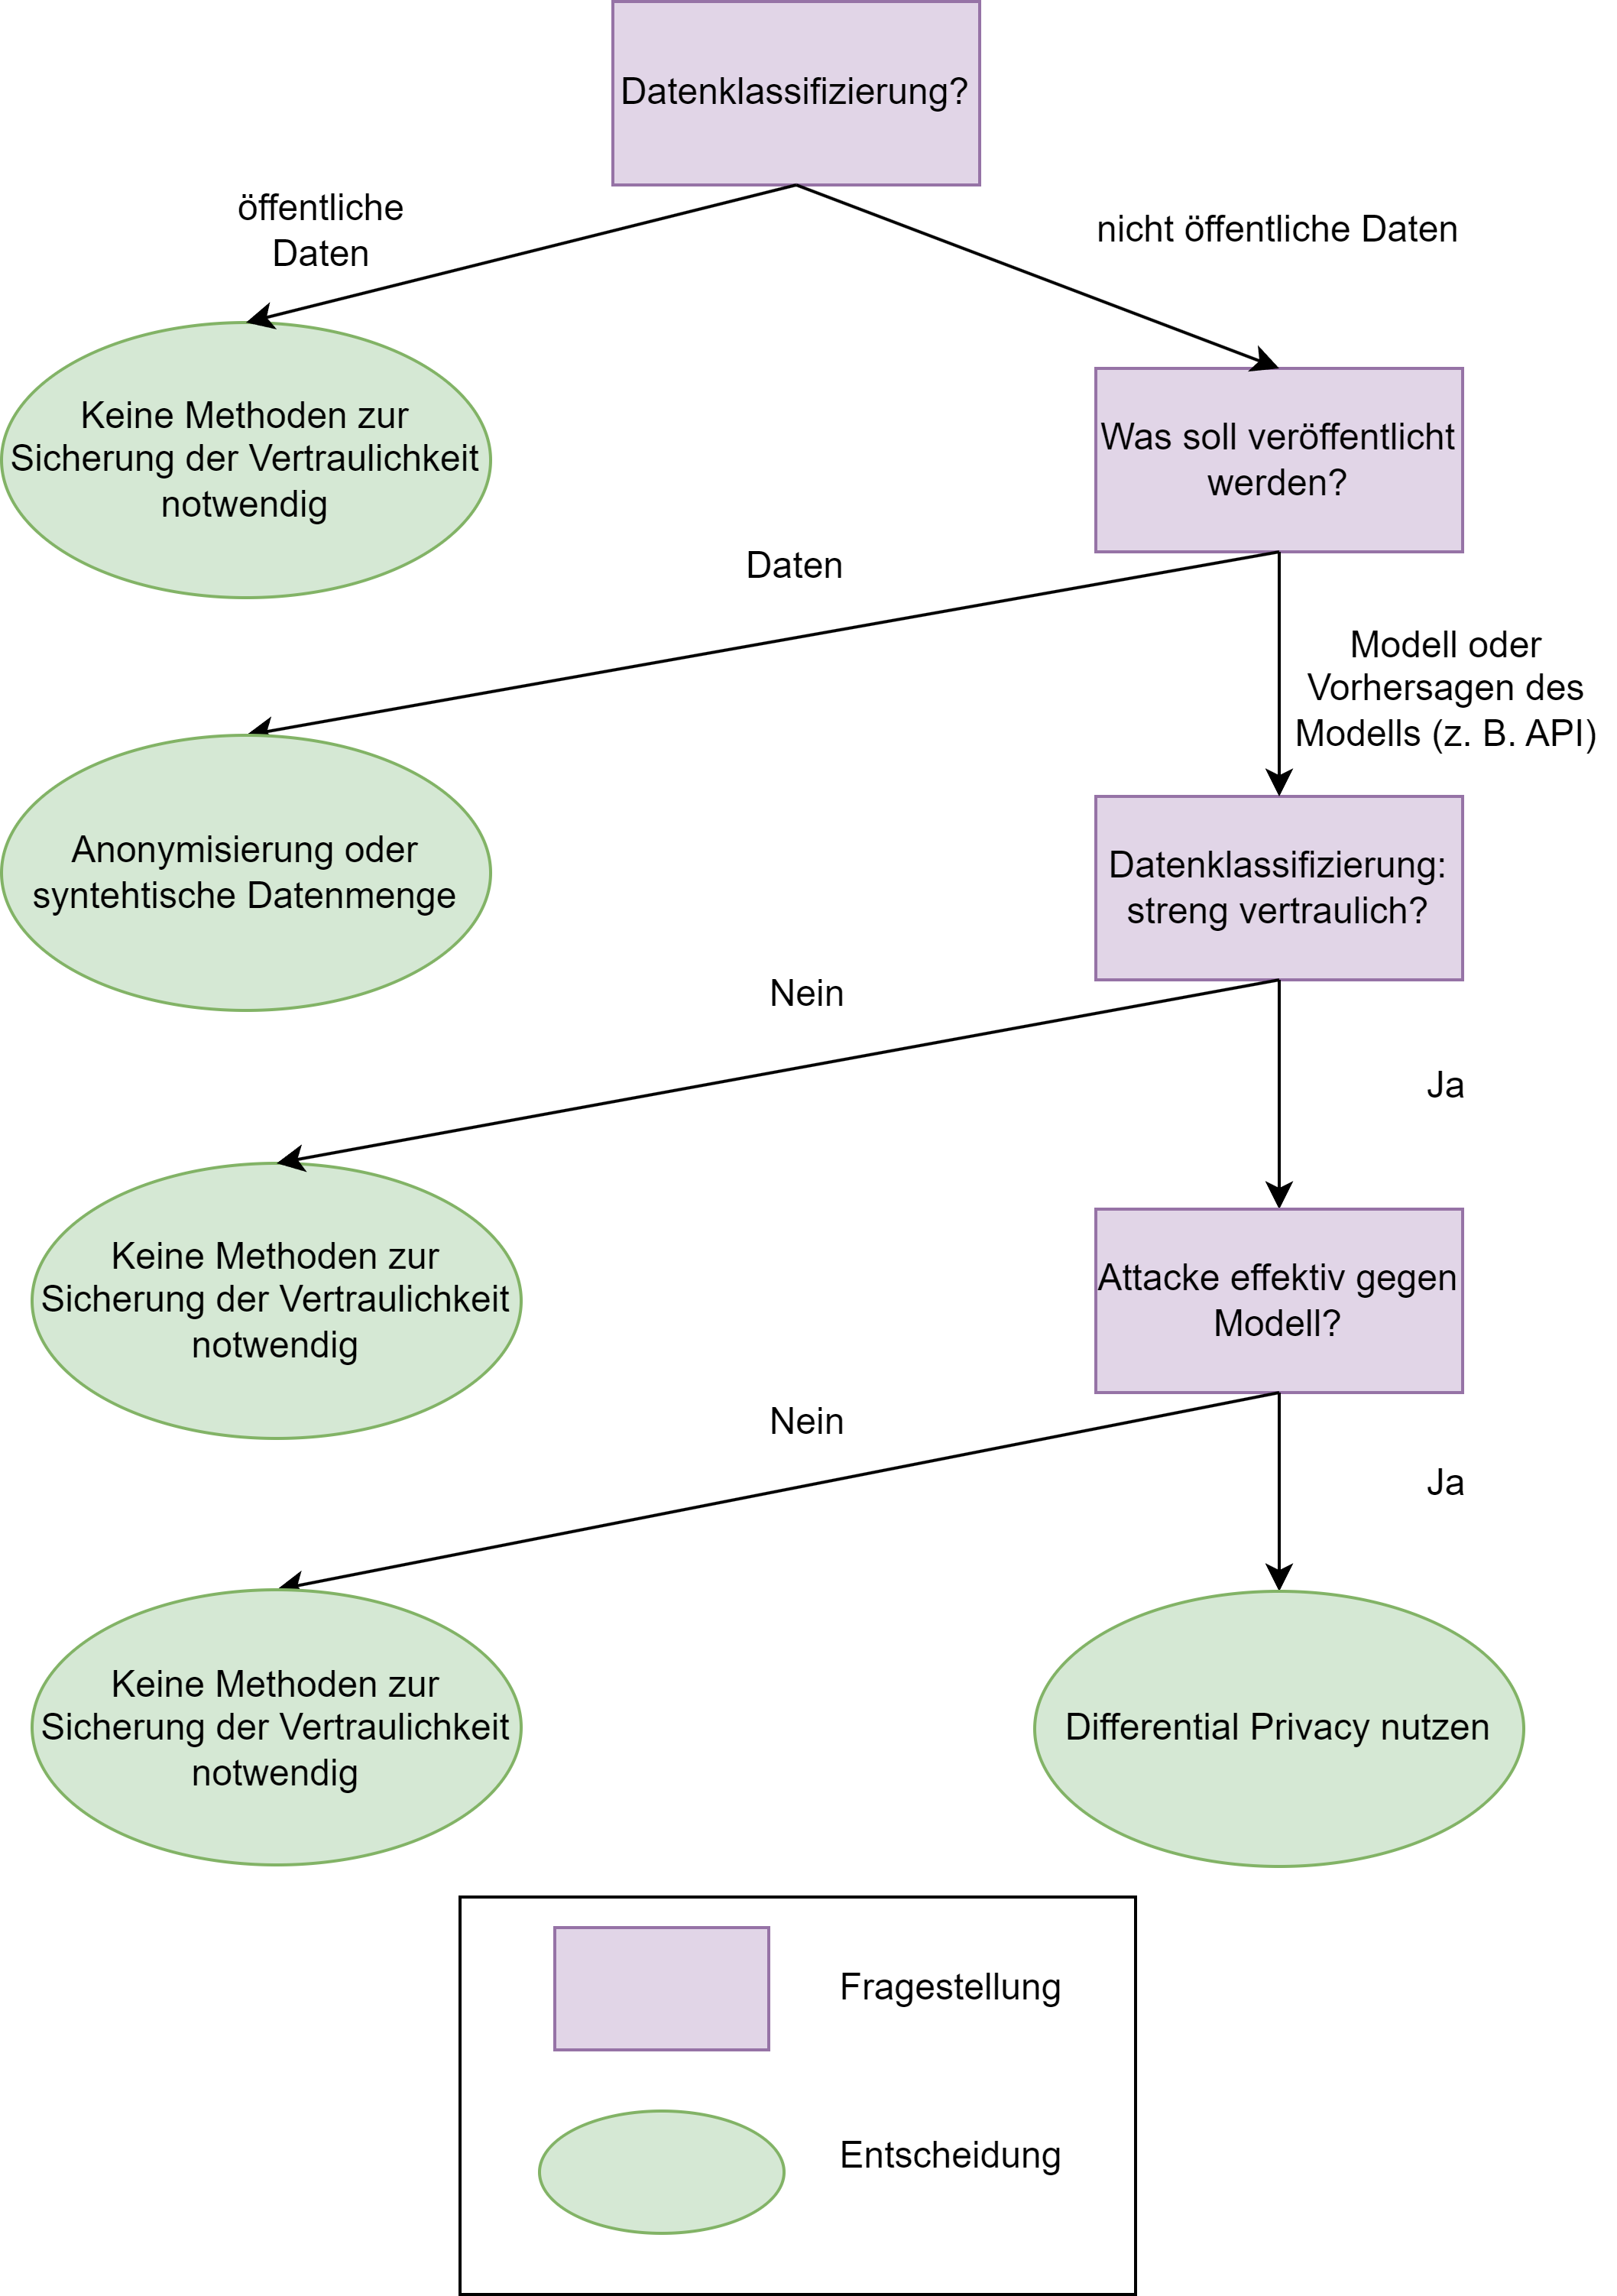
\includegraphics[width=14cm]{figures/Entscheidungsbaum.png}
    \caption{Abgleitetes Handlungsmodell}
    \label{fig:handlungsmodell}
\end{figure} 

Wird eine Anwendung auf Basis öffentlicher Daten entwickelt, ist es nicht notwendig, Methoden zur Sicherung der Vertraulichkeit zu nutzen.
Sind die Daten jedoch nicht öffentlich, hängt die Entscheidung von weiteren Faktoren ab.
Sollen die Daten selbst veröffentlicht werden, dann muss jede Art von nicht-öffentlichen Daten anonymisiert werden. 
Bei vertraulichen oder streng vertraulichen Daten, wie beispielsweise Kundendaten, gibt es die Möglichkeit synthetische Datenmengen zu erzeugen und nur diese zu veröffentlichen.

Werden nicht die Daten veröffentlicht, sondern nur das Modell oder die Vorhersagen des Modells, dann benötigen interne und vertrauliche Informationen ebenfalls keine Methoden zur Sicherung der Vertraulichkeit.
Dies liegt daran, dass die Angriffe gegen neuronale Netze nicht sehr effektiv sind. 
Experimente in Kapitel \ref{sec:exp_angriffe} zeigen dies und zusätzlich wird in Kapitel \ref{sec:dis_angriffe} die Effektivität von Angriffen diskutiert.

Da die Nutzung von streng vertrauliche Daten für ein enormes Risiko sorgt, sollten Modelle, die diese Daten nutzen, experimentell angegriffen werden.
Dies gleicht einem Penetrationstest, wobei nicht nur Schwachstellen im Anwendungscode und der Infrastruktur evaluiert werden, sondern zusätzlich noch das Modell selbst.
Die Evaluation der Angriffe kann beispielsweise automatisiert in die Deployment-Pipeline integriert werden.
Wird das Modell veröffentlicht, sollte mindestens ein White-Box Angriff evaluiert werden.
Wird das Modell lediglich über eine API bereitgestellt, reicht es, einen Black-Box Angriff zu evaluieren.
Mögliche Angriffe sind hier die Membership Inference Attacke als Black-Box Angriff und die Model Inversion Attacke als White-Box Angriff.

Bei der Effektivität der Membership Inference Attacke kann ein Schwellwert von beispielsweise 80 \% als Ziel gesetzt werden. 
Diesen Wert gilt es zu unterschreiten. 
Sollte ein Modell weniger anfällig für diesen Angriff sein, bedarf es keiner weiteren Methoden.
Liegt die Effektivität des Angriffs jedoch über dem Schwellwert von 80 \%, sollte Differential Privacy genutzt werden.
Hier empfiehlt sich die Nutzung von DPSGD oder das Verrauschen der Ausgabe.
Die Hyperparameter von DPSGD können anhand von Kapitel \ref{sec:hyperparams} optimiert werden, wobei zunächst ein hoher $\epsilon$-Wert von 50 gewählt wird.
Liegt die Effektivität des Angriffs anschließend immer noch über dem Schwellwert, sollte der $\epsilon$-Wert sukzessiv verkleinert werden.

Um eine Model Inversion Attacke zu evaluieren, benötigt es eine Möglichkeit, zu evaluieren, ob ein rekonstruierter Datensatz einem originalen Datensatz ähnelt.
Dies könnte über mathematische Metriken, \zB mittels der Kosinus-Ähnlichkeit zweier Vektoren, bewertet werden, ohne von menschlichen Fachexperten beurteilt werden.
Mathematische Metriken bieten den Vorteil, dass hier ein Schwellwert festgelegt werden kann, wohingegen dies bei einer menschlichen Beurteilung nicht möglich ist.
Ist die Effektivität des Angriffs hoch, sollte hier ebenfalls Differential Privacy genutzt werden.


